\section{Luminosity Determination}

Our statistical uncertainties on $A_{LL}$ assume perfect knowledge of the
relative luminosity of the different spin states. This systematic addresses
that simplification.

\subsection{Uncertainty Evaluation Using the ZDCs}

% \textit{Note: \href{http://mare.tamu.edu/star/2005n06Jets/2005relLumSys_mar29_2008/}{analysis by Murad Sarsour}}

We can quantify the precision with which we understand the relative luminosities
obtained from the BBCs by using an independent luminosity monitor, the ZDCs. In
the absence of non-statistical fluctuations, the uncertainty on R will be
dominated by the statistics in the ZDCs, which count at a much lower rate than
the BBCs during proton-proton running.

A couple of problems in the ZDC data need to be corrected before a comparison
to the BBCs can be trusted. The first problem is due to the ``killer bit''
algorithm, which suppressed signals in the ZDCs for 10 bunch crossings after
an initial signal. The algorithm is used in heavy ion running to prevent
ringing in the calorimeters from generating false signals, but in pp running
it biases the ZDC counts. Bunch crossings immediately following abort gaps
(where the killer bit is more likely to be off) end up with more ZDC counts
than crossings in the middle of a filled set of bunches. As a result, the
ratio of relative luminosities obtained from the ZDC and BBC will not be flat,
see Figure \ref{fig:zdctobbc6170012zoom}.

\begin{figure}
  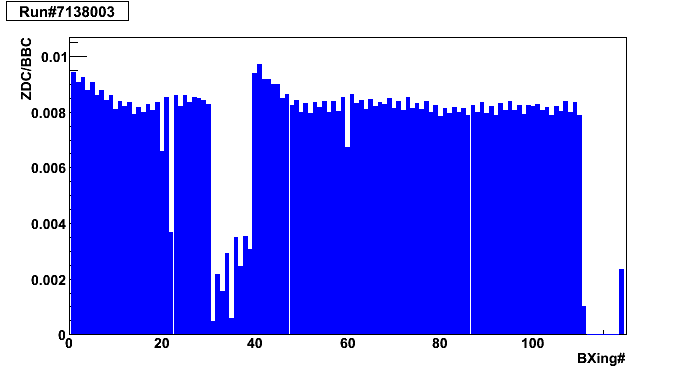
\includegraphics[width=1.0\textwidth]{figures/ZDCtoBBC_r7138003}
  \caption{Ratio of ZDC and BBC counts versus bunch crossing.  Notice that the ratio is larger in bunch crossings immediately following abort gaps.}
  \label{fig:zdctobbc6170012zoom}
\end{figure}

The procedure developed to correct for this effect requires scaling the counts
for a given bunch crossing by a factor that takes into account the frequency
with which the previous ten bunch crossings had a signal. For the ZDC singles
rates, the formula for the corrected counts $n_{j}$ in a given bunch crossing
$j$ is
%
\begin{equation}
  n_{j}^{corrected} = n_{j} * \frac{N_{cycles}}{N_{cycles} - \sum_{i=1}^{10}n_{j-i}}
\end{equation}
%
where $N_{cycles}$ is the number of times the beam cycled through STAR in the
run. Figure \ref{fig:zdc-singles-ratio} shows the effect of applying the
correction for a sample run.

\begin{figure}
  \subfigure{
    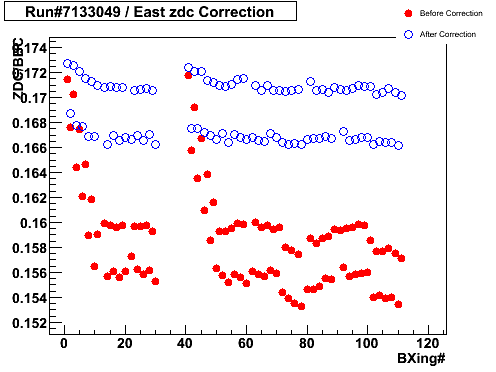
\includegraphics[width=0.5\textwidth]{figures/ZDCtoBBC_r7133049ER}
  }
  \subfigure{
    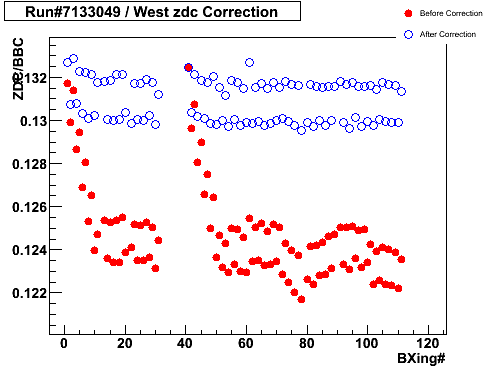
\includegraphics[width=0.5\textwidth]{figures/ZDCtoBBC_r7133049WR}
  }
  \caption{Change in the ZDC singles rates after applying the killer bit correction.}
  \label{fig:zdc-singles-ratio}
\end{figure}

The formula to correct the ZDC coincidence counts is complicated by the need
to track the killer bits for the two detectors simultaneously. The formula for
the corrected coincidence counts $c_{j}$ given singles counts $e_{j}$ (ZCDE)
and $w_{j}$ (ZDCW) is
%
\begin{align}
  &\alpha_{j} = N_{cycles} - \sum_{i=1}^{10}c_{j-i} \notag\\
  &\beta_{j} = \sum_{i=1}^{10}(e_{j} + w_{j} - 2*c_{j}) - \sum_{i=1}^{9}\left[\frac{(e_{j}-c_{j}) * (w_{j}-c_{j})}{\alpha_{j}-(e_{j-10}-c_{j-10})} + \frac{(e_{j}-c_{j}) * (w_{j}-c_{j})}{\alpha_{j}-(w_{j-10}-c_{j-10})}\right] + ... \notag\\
  &c_{j}^{corrected} = c_{j} * \frac{N_{cycles}}{\alpha_{j} - \beta_{j}} 
\end{align}
%
and the effect of the killer bit correction on the coincidence distributions
is shown in Figure \ref{fig:coinRat6143016}

\begin{figure}
  \begin{center}
    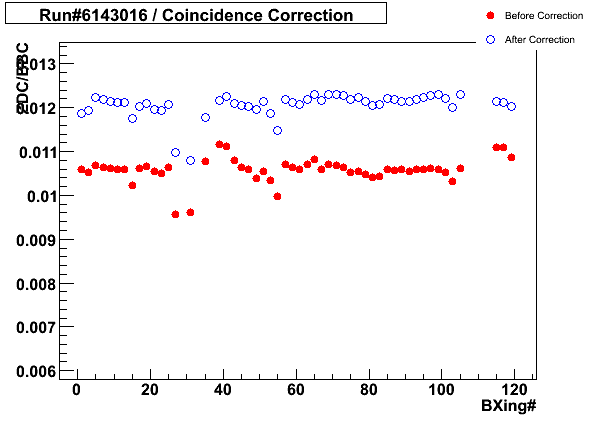
\includegraphics[width=0.6\textwidth]{figures/coinRat6143016}
  \end{center}
  \caption{Change in the ZDC coincidence rates after applying the killer bit
  correction.}
  \label{fig:coinRat6143016}
\end{figure}

\begin{figure}
  \begin{center}
    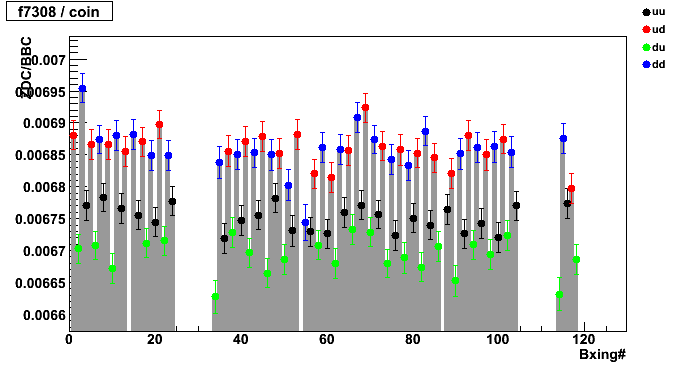
\includegraphics[width=0.8\textwidth]{figures/c7308}
  \end{center}
  \caption{Example of a coherent spin pattern and even-odd ZDC rate
  oscillation. In this case, the ZDC rate is always higher when the spin of
  the blue beam is down.}
  \label{fig:c7308}
\end{figure}

The second problem that we need to correct has come to be known as the
``even-odd'' effect. It turns out that the ZDC coincidence rates are often
different for even-numbered and odd-numbered bunch crossings. This oscillation
can introduce a false asymmetry if it aligns coherently with a particular spin
pattern. For instance, in Figure \ref{fig:c7308} we see that the ZDC
coincidence rates are always higher when the spin of the blue beam is down.
Figure \ref{fig:fevfod} shows the time dependence of this even-odd
oscillation, with the colors now representing individual fills. To quantify
the bias this introduces on $A_{LL}$, we can define the fractional overlap
between the even-odd ZDC oscillation and relevant portion of the spin pattern
for $A_{LL}$ using a 120 element vector $|EO\rangle = |+1,-1,+1,-1,...\rangle$
and another 120 element vector $|LL\rangle$ whose elements are 1 if the bunch
crossing is UU or DD, -1 if UD or DU, and 0 otherwise. The inner product of
these vectors measures the susceptibility of $A_{LL}$ for that spin pattern to
any even-odd oscillation.

\begin{figure}
  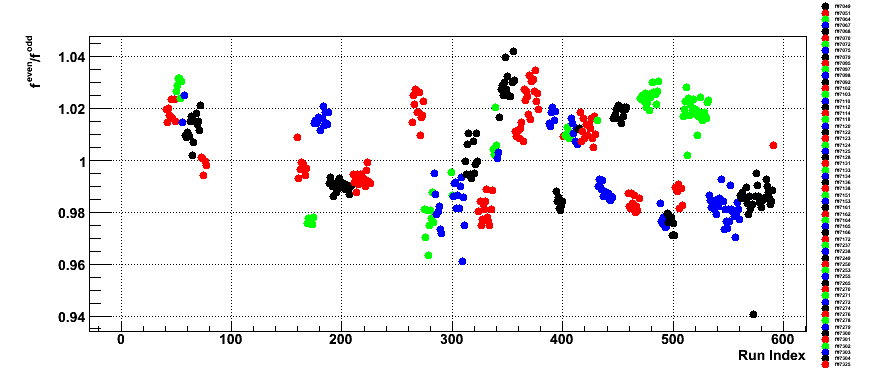
\includegraphics[width=1.0\textwidth]{figures/fevfod}
  \caption{Magnitude of even-odd rate asymmetry versus time.}
  \label{fig:fevfod}
\end{figure}

It turns out that $A_{LL}$ is less biased by the even-odd rate oscillation in
the ZDC than, say, the blue beam single-spin asymmetry. Figure \ref{fig:cll}
plots the fill-by-fill change in $A_{LL}$ if the ZDC is used for relative
luminosities instead of the BBC against the the product of the fractional
overlap $F \equiv \langle EO | LL \rangle$ and the magnitude of the even-odd
oscillation $S-1$. Placing a cut on $|F*(S-1)| < 0.002$ is well-motivated. For
fills without reliable ZDC information, we use Figure \ref{fig:fevfod} to
assume a conservative $|S-1| = 0.03$.

\begin{figure}
  \begin{center}
  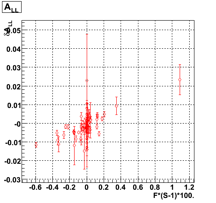
\includegraphics[]{figures/cll}
  \end{center}
  \caption{Change in $A_{LL}$ versus the product of the even-odd rate oscillation amplitude and the fractional overlap $\langle EO | LL \rangle$.  Deviations from 0 on the x-axis indicate fills where $A_{LL}$ is biased by the even-odd effect.}
  \label{fig:cll}
\end{figure}

After correcting for the killer bits and rejecting the fills that fail the
even-odd oscillation cut the uncertainty on $A_{LL}$ due to the uncertainty in
the relative luminosities is estimated to be $9.32\times10^{-4}$.

\subsection{Beam Background Bias}

\textit{Note: \href{http://www.star.bnl.gov/protected/spin/kowalik/2005/r-lumi/bkg_sys.html}{analysis by Kasia Kowalik}}

The relative luminosities obtained from the BBCs might also be biased by false
signals generated by beam-gas background. We can try to quantify this by
studying the coincidence rate in crossings where one of the two beams has an
unfilled bunch (``abort gaps''). The beam-gas background is assumed to be
crossing- and spin-independent, but it can be different in each beam. It
follows that the per-crossing coincidence rate due to beam-gas in each beam is
just the average number of BBC coincidences found in the abort gaps for that
beam. In Figure \ref{fig:bkg-yellow-blue}, the x-axis is the background rate
divided by the total rate, defined as the average number of coincidences per
bunch crossing with a spin state of UU, UD, DU, or DD. The two histograms are
incremented for each STAR run. We see that the background rate in the BBCs due
to beam-gas is typically less than 0.1\% of the total rate.

\begin{figure}
  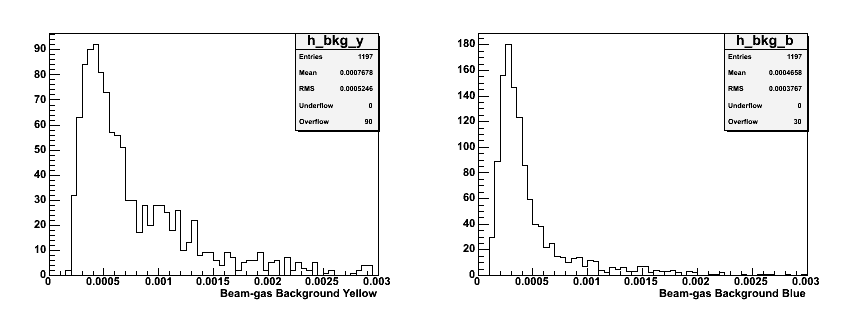
\includegraphics[width=1.0\textwidth]{figures/bkg-yellow-blue}
  \caption{Fraction of the total coincidence rate attributed to beam gas in
  each beam. The histograms are incremented once for each STAR run.}
  \label{fig:bkg-yellow-blue}
\end{figure}

Given run-dependent background fractions for both beams, it's possible to
calculate background-subtracted relative luminosities. Figure
\ref{fig:r-lumi-sys-bkg} shows the difference between the raw relative
luminosity and the background-subtracted version. The background-corrected
relative luminosities yield an $A_{LL}$ that differs from the original by
$3.0\times10^{-4}$, so we use that as the uncertainty for this source of
systematic error.

\begin{figure}
  \begin{center}
    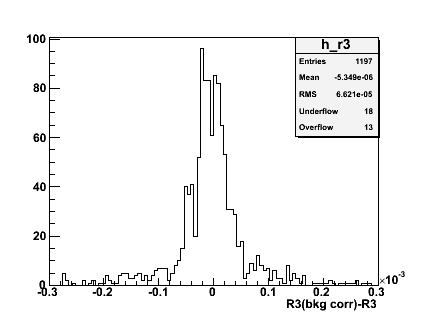
\includegraphics[width=0.6\textwidth]{figures/r-lumi-sys-bkg}
  \end{center}
  \caption{Change in the relative luminosities after correcting for beam-gas
  background.}
  \label{fig:r-lumi-sys-bkg}
\end{figure}
